
%%%%%%%%%%%%%%%%%%%%%%% file typeinst.tex %%%%%%%%%%%%%%%%%%%%%%%%%
%
% This is the LaTeX source for the instructions to authors using
% the LaTeX document class 'llncs.cls' for contributions to
% the Lecture Notes in Computer Sciences series.
% http://www.springer.com/lncs       Springer Heidelberg 2006/05/04
%
% It may be used as a template for your own input - copy it
% to a new file with a new name and use it as the basis
% for your article.
%
% NB: the document class 'llncs' has its own and detailed documentation, see
% ftp://ftp.springer.de/data/pubftp/pub/tex/latex/llncs/latex2e/llncsdoc.pdf
%
%%%%%%%%%%%%%%%%%%%%%%%%%%%%%%%%%%%%%%%%%%%%%%%%%%%%%%%%%%%%%%%%%%%


\documentclass[runningheads,a4paper]{llncs}

\usepackage[utf8]{inputenc}
\usepackage[T1]{fontenc}
\usepackage{caption}
\usepackage{subcaption}
\usepackage{amssymb}
\setcounter{tocdepth}{3}
\usepackage{graphicx}
\graphicspath{ {./images/} }
\usepackage{hyperref}
\usepackage{url}
\usepackage{listings, chngcntr}
\usepackage{color}
\definecolor{lightgray}{rgb}{.9,.9,.9}
\definecolor{darkgray}{rgb}{.4,.4,.4}
\definecolor{purple}{rgb}{0.65, 0.12, 0.82}

\lstdefinelanguage{JavaScript}{
  keywords={typeof, new, true, false, catch, function, return, null, catch, switch, var, if, in, while, do, else, case, break},
  keywordstyle=\color{blue}\bfseries,
  ndkeywords={class, export, boolean, throw, implements, import, this},
  ndkeywordstyle=\color{darkgray}\bfseries,
  identifierstyle=\color{black},
  sensitive=false,
  comment=[l]{//},
  morecomment=[s]{/*}{*/},
  commentstyle=\color{purple}\ttfamily,
  stringstyle=\color{red}\ttfamily,
  morestring=[b]',
  morestring=[b]"
}

\lstset{
   language=JavaScript,
   extendedchars=true,
   basicstyle=\footnotesize\ttfamily,
   showstringspaces=false,
   showspaces=false,
   numbers=left,
   numberstyle=\footnotesize,
   numbersep=9pt,
   tabsize=2,
   breaklines=true,
   showtabs=false,
   captionpos=b
}

\renewcommand{\lstlistlistingname}{List of Listing}

\newcommand{\keywords}[1]{\par\addvspace\baselineskip

\noindent\keywordname\enspace\ignorespaces#1}

\begin{document}

\counterwithout{lstlisting}{section}

\mainmatter  % start of an individual contribution

% first the title is needed
\title{TypeDevil: Dynamic Type Inconsistency Analysis for JavaScript\\-\\Seminar Report}

% a short form should be given in case it is too long for the running head
\titlerunning{TypeDevil - Seminar Report}

% the name(s) of the author(s) follow(s) next
\author{Nico Fechtner}
%
\authorrunning{Seminar Report: TypeDevil}
% (feature abused for this document to repeat the title also on left hand pages)

% the affiliations are given next; don't give your e-mail address
% unless you accept that it will be published
\institute{Technical University of Munich\\
Department of Informatics\\
Chair for IT Security\\
Boltzmannstraße 3, 85748 Garching, Germany\\
\href{mailto:nico.fechtner@tum.de}{nico.fechtner@tum.de}
}

%
% NB: a more complex sample for affiliations and the mapping to the
% corresponding authors can be found in the file "llncs.dem"
% (search for the string "\mainmatter" where a contribution starts).
% "llncs.dem" accompanies the document class "llncs.cls".
%
% ???
\toctitle{}
\tocauthor{}
\maketitle
 \newpage
 \thispagestyle{empty}
\begin{abstract}
    JavaScripts dynamic and weak type system makes it possible to write type inconsistent and therefore buggy code. 
    TypeDevil addresses this issue with a mostly dynamic type inconsistency analysis which is able to effectively warn developers about critical type related bugs.
    An alternative solution heavily used in the industry are additional static type system like e.g. TypeScript.
    A comparative evaluation shows that both approaches perform quite similar in identifying type inconsistencies with TypeScript being about 14\% better at finding true positives.
    %\keywords{Dynamic Type Inconsistency Analysis for JavaScript, TypeDevil, Static Type Systems for JavaScript, TypeScript}
    \end{abstract}
    
    \newpage

\setcounter{tocdepth}{2}
\tableofcontents
\newpage
\lstlistoflistings % The list of listings
\newpage

\section{Introduction}

This report is part of the seminar "Common Security Flaws in JavaScript based Applications" \cite{CommonSecFlaws}, which was held by Paul Muntean from the Chair of IT Security at the Faculty of Informatics of the Technical University of Munich.
The seminar took place in the summer semester 2018 and dealt with several scientific papers related to JavaScript Security. \\
The paper I took a deeper look at is "TypeDevil: Dynamic Type Inconsistency Analysis for JavaScript" \cite{DBLP:conf/icse/PradelSS15}, published in 2015 by Michael Pradel, Parker Schuh and Koushik Sen.
This report illustrates the general problem the paper tries to address, introduces TypeDevil as a possible solution and compares it to an alternative approach, namely additional static type systems. 

\section{Inconsistent Types as the Root Cause of Many Bugs}
First of all, let me introduce the general problem that TypeDevil tries to solve. \\
JavaScript was developed by Brendan Eich back in 1995 in about ten days and was - as the name suggests - originally just intended for small inline scripts.
However, these days there are critical business applications like banking front-ends written entirely in JavaScript. 
Being one of today's most popular programming languages, JavaScript features two striking characteristics this report will focus on. 
On the one hand, JavaScript is dynamically typed. 
This basically means, that developers do not provide any static type annotations to their source code, like you would do in statically typed languages, such as e.g. Java, and that types - for example of local variables - can change during runtime.
On the other hand, JavaScript is also weakly typed and thereby very permissive. In order to prevent runtime exceptions, JavaScript performs a lot of automatic type conversions, also known as implicit coercions.
Consider the code example in listing \ref{listingPets}. 
One could expect the script to print \lstinline[columns=fixed]{"Cat Dog Rabbit "} to the console.
The actual output however is \lstinline[columns=fixed]{"undefinedCat Dog Rabbit "}. 
In the first iteration of the for-loop, it is being attempted to concatenate a string to the value of \lstinline[columns=fixed]{outputString}, which is undefined. 
JavaScript now performs a implicit coercion and converts the value \lstinline[columns=fixed]{undefined} to the string \lstinline[columns=fixed]{"undefined"} which leads to the unexpected output.

\medskip\medskip
\lstset{language=javascript}
\begin{minipage}{\linewidth}
\begin{lstlisting}[frame=single, caption=Implicit Coercions, label={listingPets}] 
var pets = ["Cat", "Dog", "Rabbit"];

var outputString;

for (var i in pets) {
    outputString += pets[i] + " ";
}

console.log(outputString);
\end{lstlisting}
\end{minipage}

As pointed out above, dynamic languages do not require programmers to annotate their programs with type information or to follow any strict typing discipline. 
This freedom allows developers to write concise code in short time. 
However, most code does follow implicit type rules, e.g. only a single type per variable or object property or fixed function signatures.
The authors of TypeDevil further state that many bugs are actually violations of these rules.
So the freedom offered by dynamic languages often comes at the cost of hidden bugs and since the language does not enforce any typing discipline, no compile-time warnings are reported if a program uses and combines types inconsistently.
Although the code example does not seem that harmful, when you consider business sensitive services like authentication or payment libraries, of course even a little type error could do some real damage. \\
TypeDevil wants to address this problem by gathering type observations during run-time, summarizing them into a type graph and finally reporting a set of aggressively filtered type inconsistency warnings.
The challenges are on the one hand the absence of static type information and on the other hand the fact that a lot of JavaScript code is polymorphic on purpose and the tool shouldn't report false positives when encountering intended polymorphic constructs.

\section{Static and Dynamic Analyses} \label{staticDynamicAnalysis}

For better understanding of the following the difference between static and dynamic analyses should be clarified first.\\
The key differentiation point is that within a static analysis you do not have any runtime information, since the analysis runs ahead of time and the only input to the analysis is the source code itself.
Therefore it is usually quite hard to predict the exact program behavior.
It turns out, that it is even harder to get comprehensive and precise results for dynamic languages like JavaScript, because of constructs like the \lstinline[columns=fixed]{eval()} function, which interprets the string passed to it at runtime as normal JavaScript code. 
However the advantage of static analysis is that it usually covers all code paths and runs quite fast.
Typical examples for static analyses in the context of JavaScript are linters, like ESLint, JSLint or Prettier, which are capable of ensuring that certain best practices are followed and detecting common programming errors. \\
Dynamic analyses are typically characterized by the ability that they do have access to runtime information.
Often, instrumentation code is added to the original source code to track certain features of the program that are relevant to the analysis.
After that, this instrumented version of the source code gets executed, the analysis gathers runtime information, e.g. user input, and the results of the analysis get computed.
With this approach you can catch certain errors, static analysis would not be able to find.
For example, consider again the \lstinline[columns=fixed]{eval()} function, where dynamic analyses can be able to track the code which gets interpreted on the fly.
However, the biggest downside of a purely dynamic analysis is, that it can not cover all code paths most of the time.
The following section will focus on TypeDevils mostly dynamic approach to gather type observations at runtime.

\section{TypeDevils Approach}

This section will introduce the core mechanisms TypeDevil uses to effectively identify and report inconsistent types.
There is a prototype of TypeDevil implemented by the authors on top of Jalangi \cite{DBLP:conf/sigsoft/SenKBG13a} which can be found on GitHub \cite{TypeDevilGitHub}.\\
In general, there are three main phases, TypeDevil goes through: 
First, instrumentation code gets inserted to the original source code to gather type observations at every relevant code location and subsequently the instrumented program gets executed.
From this potentially huge amount of type observations, TypeDevil constructs a type graph that makes it relatively easy to summarize types that are structurally equivalent.
On the basis of the condensed type graph, TypeDevil identifies inconsistent types and applies a set of merging and pruning techniques to drastically reduce the number of reported warnings and false positives, respectively.

\subsection{Running Example}
Listing \ref{listingRunningExample} shows the running example used to introduce the various steps of TypeDevils pipeline.
This is also the example the original TypeDevil paper used to illustrate the various techniques.
First, there is a simple function \lstinline[columns=fixed]{addWrapped} which takes two arguments and returns the addition of the \lstinline[columns=fixed]{v} properties of both arguments if the function receives two parameters and returns just the \lstinline[columns=fixed]{v} property of the first argument if only one parameter is passed.
Then there is a simple constructor function \lstinline[columns=fixed]{Wrapper} which - when called with the \lstinline[columns=fixed]{new} keyword - creates an object with a single property \lstinline[columns=fixed]{v}.
Lastly \lstinline[columns=fixed]{addWrapped} gets called three times with different parameters.
Of course it sticks out that the \lstinline[columns=fixed]{v} property of the object which gets passed to \lstinline[columns=fixed]{addWrapped} when calling it the third time is a string and not a number.
This seems to be a type inconsistency and it will turn out that TypeDevil can effectively warn programmers about this problem.

\medskip\medskip
\lstset{language=javascript}
\begin{minipage}{\linewidth}
\begin{lstlisting}[frame=single, caption=Running Example, label=listingRunningExample]
function addWrapped(x, y) {
    if (y) {
        return x.v + y.v;
    } else {
        return x.v;
    }
}

function Wrapper(v) {
    this.v = v;
}

addWrapped({v:23});
addWrapped({v:20}, new Wrapper(3));
addWrapped({v:"18"}, new Wrapper(5));
\end{lstlisting}
\end{minipage}


\subsection{Gathering Type Observations}

The first phase of TypeDevil is to gather type observations at runtime.
To achieve this, TypeDevil first off automatically instruments the original source code in two ways.
On the one hand, a shadow value gets added to each object and function, containing a unique identifier, which makes it easy to access the objects of functions type name whenever they are referred to. 
On the other hand, TypeDevil saves type observations at every relevant code location to a global set.
In the sense of TypeDevil, a type is either a primitive type (boolean, number, string, undefined, null) or a so called record type, which basically maps a named property to a set of types.
For record types, TypeDevil differentiates between object types, array types, function types and (function) frame types.
A type observation is therefore a triple consisting of a basetype, a property and an observed type.
After instrumenting the original source code, TypeDevil executes the program and dynamically gathers type observations which results in a huge set of these observations for further processing.
The authors of TypeDevil implemented two versions of the analysis. 
It can either be run on top of node or a custom version of Firefox with a modified version of Spidermonkey, the JavaScript engine of Firefox, can be used.
In the following, each code construct TypeDevil instruments ahead of time will get explained.

\subsubsection{Object Literals}
Consider \lstinline[columns=fixed]{addWrapped} gets called for the first time.
With the object literal \lstinline[columns=fixed]!{v:23}! a new object gets created to pass it to the function.
First, a shadow value holding a unique identifier get appended to the newly created object. A possible unique identifier could just be the string \lstinline[columns=fixed]{"object"} concatenated with a unique number, e.g. \lstinline[columns=fixed]{"object1"}.
After that, a type observation for each property of the object gets added to the global set of observations.
In the example the type observation \lstinline[columns=fixed]{(object1, v, number)} would be added, since \lstinline[columns=fixed]{"object1"} is the basetype, \lstinline[columns=fixed]{v} is the name of the property and \lstinline[columns=fixed]{23} is a numeric value.

\subsubsection{Property Access}
TypeDevil also gathers type observations on each property access.
In the example, when \lstinline[columns=fixed]{addWrapped} gets called for the first time, there is no second argument provided, so the execution will definitely end up in the else branch on line 5. 
There the property \lstinline[columns=fixed]{v} of the passed object gets accessed.
So TypeDevil adds the type observation \lstinline[columns=fixed]{(object1, v, number)}.
As you can see, this is exactly the same type observation which was already stored at the creation of the object which seems quite redundant at the first glance. 
Nevertheless TypeDevil has to add a type observation for each property access, since code which does not get instrumented like third party libraries or code which just cannot get instrumented, namely native code, could potentially change the types of properties.

\subsubsection{Function Literals}
Just as with objects, TypeDevil also appends shadow values containing unique identifiers to all function literals.
In the example, it would append the unique identifier \lstinline[columns=fixed]{"function addWrapped"}, to the function starting at line 1.

\subsubsection{Function Calls}
For each function call, TypeDevil adds two type observations.
The first one refers to the receiver of the function and the second one refers to the return type.
Consider again the first call of \lstinline[columns=fixed]{addWrapped}.
TypeDevil adds the type observation \lstinline[columns=fixed]{(function addWrapped, this, window)}, since \lstinline[columns=fixed]{addWrapped} gets called without an explicit receiver in which case the global object - e.g. \lstinline[columns=fixed]{window} - becomes the receiver
and \lstinline[columns=fixed]{(function addWrapped, return, number)}, since the function returns a numeric value (\lstinline[columns=fixed]{23}).

\subsubsection{Variable Access}
Analogical to property accesses, TypeDevil deals with local variable accesses.
It is important to note, that similar to the internal implementation of JavaScript itself, TypeDevil treats function arguments as local variables.
Like in the previous examples, consider the first call of \lstinline[columns=fixed]{addWrapped}.
TypeDevil adds the type observation \lstinline[columns=fixed]{(frame addWrapped, y, undefined)} when the value of \lstinline[columns=fixed]{y} gets accessed, which happens to be \lstinline[columns=fixed]{undefined}.


\subsection{Building the Type Graph and Identifying Inconsistent Types}
\label{TGs}
Having gathered a big set of type observations, TypeDevil - while iterating over each observation - is able to produce a type graph using the following heuristic.
In the first step, every type becomes a node in the graph.
If a type is a record type, for each property an outgoing edge is added labeled with the name ofthe property and directing to the type of this property. 
There is only one node for each occurring primitive type.
Figure \ref{fig:UncondensedTG} shows the uncondensed type graph resulting from this heuristic for the running example.\\
Subsequently, TypeDevil condenses the graph, so that there are no two nodes which are structurally equivalent, which means there are no nodes left which have outgoing edges equally labled and pointing to the same type.
Figure \ref{fig:CondensedTG} shows the condensed type graph for the running example.
E.g. \lstinline[columns=fixed]{object1}, \lstinline[columns=fixed]{object2}, \lstinline[columns=fixed]{object3} and \lstinline[columns=fixed]{object5} were merged together, since they are structurally equivalent.
Condensing the type graph is extremely important, because the redundancy of the initial graph can really slow down the following operations on the graph. \\
TypeDevil can now identify inconsistent types. 
The intuition is again quite simple: 
Whenever a type has got two or more outgoing edges, labeled equally, but pointing to different types, there is a type inconsistency.
In the running example, the local variables \lstinline[columns=fixed]{x} and \lstinline[columns=fixed]{y} are obviously of inconsistent types.

\begin{figure}[h]
\fbox{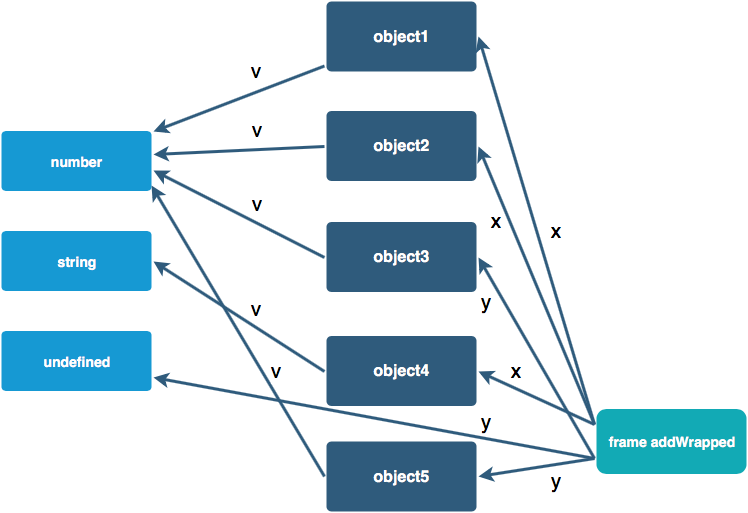
\includegraphics[width=\textwidth]{UncondensedTG}}
\caption{Uncondensed Type Graph}
\label{fig:UncondensedTG}
\end{figure}

\begin{figure}[h]
\fbox{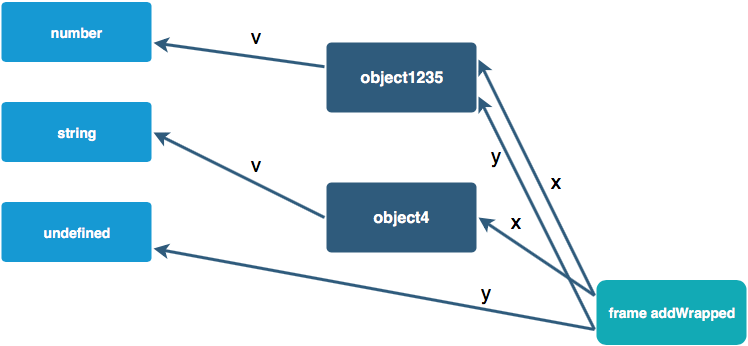
\includegraphics[width=\textwidth]{CondensedTG}}
\caption{Condensed Type Graph}
\label{fig:CondensedTG}
\end{figure}


\subsection{Merging and Pruning of Warnings}

A naive implementation of the approach explained in \ref{TGs} reports various false positives, since a variable, property, or function may refer to multiple types on purpose. 
TypeDevil combines two kinds of techniques to distinguish such intended polymorphic code from actual inconsistency problems. 
First of all, the authors of TypeDevil developed techniques which try to group warnings which seem to have the same root cause in the same equivalence class.
In a second step, TypeDevil marks warnings which are likely to be false positives for pruning.
In the end, only one warning per equivalence class is kept only if none of the warnings in this class are marked for pruning.\\
\cite{DBLP:conf/icse/PradelSS15} describes the following unique heuristics:
\begin{itemize}
    \item Merging by dataflow relations
    \item Merging by type diff
    \item Merging by array type
    \item Pruning by belief analysis
    \item Pruning by degree of inconsistency
    \item Pruning by size of type diff
    \item Pruning of structural subtypes
    \item Pruning of \lstinline[columns=fixed]{null}-related warnings
  \end{itemize}
Definitely the most interesting technique is pruning by belief analysis which utilizes a static analysis taking place before the main dynamic analysis of TypeDevil and should be described in the following.\\
Consider listing \ref{lst:BeliefAnalysis} which is taken from \cite{DBLP:conf/icse/PradelSS15} and shows the original source code before the analysis. The comments are for explanatory purposes only and do not influence the analysis.

\medskip\medskip
\lstset{language=javascript}
\begin{minipage}{\linewidth}
\begin{lstlisting}[frame=single, caption=Pruning via Belief Analysis, label={lst:BeliefAnalysis}]
function BigInteger(a, b, c) { 
    this.array = new Array();
    if (a != null) // belief: a may be undefined or null
        if ('number' == typeof a) // belief: a may be number
            this.fromNumber(a, b, c);
        else if (b == null && // belief: b may be undefined or null
            'string' != typeof a) // belief: a may be string
            this.fromString(a, 256); 
        else  
            this.fromString(a, b);
}
\end{lstlisting}
\end{minipage}

As you can see, this script uses runtime type checks to distinguish the types that the first two parameters of \lstinline[columns=fixed]{BigInteger} may have.
This is a really common idiom in real world JavaScript code.
A naive implementation of TypeDevil would report type inconsistencies e.g. when \lstinline[columns=fixed]{BigInteger} gets called one time with the first parameter being \lstinline[columns=fixed]{null} and the second time with the first parameter being numeric, even though the program is correct. 
To avoid such false positives TypeDevil performs a static analysis to extract the programmer’s "intent".
Common idioms used to check the runtime type of a variable are recognized and the according "belief" is stored as an string expression at the beginning of the according function.
The main analysis then uses this information to prune warnings which are false positives.
E.g. for \lstinline[columns=fixed]{BigInteger}, TypeDevil would not report a warning if \lstinline[columns=fixed]{a} is sometimes \lstinline[columns=fixed]{null} and sometimes a \lstinline[columns=fixed]{number}.

\section{Static Type Systems as an Alternative to Dynamic Analysis}

Additional static type systems for JavaScript got a lot of attention over the last years, since major IT companies like Google, Facebook or Microsoft are developing them and provide production ready tools for developers.
Trying to solve basically the same problem as TypeDevil, they want to provide developers with warnings for type inconsistent code, but in contrast to dynamic analyses like TypeDevil you already get these warnings ahead of time.
Important to note is that static type systems for dynamic languages also have a lot of additional advantages.
For example they enable a mature development experience with rich auto completion, advanced refactoring options and always up-to-date code documentation.
However, in the following the focus will be on type warnings.

\subsection{Approach of Additional Static Type Systems} \label{staticTypeSystems}
There are a lot of different additional static type systems for JavaScript.
The three most used ones are TypeScript from Microsoft \cite{TypeScript}, Flow from Facebook \cite{Flow} and the Google Closure Compiler \cite{ClosureComiler}.
Basically all of them behave and work quite similar.
Usually, they are a superset of JavaScript, which means that every JavaScript program is also already for example a syntactically valid TypeScript or a Flow program.
This makes the gradual adoption of an additional type system really easy.
The basic approach is to extend the core JavaScript language with additional type annotations, either in the form of inline types (TypeScript, Flow) or in the form of special comments (Google Closure).
Another common characteristic state of the art static type checkers share is their mature type inference, which means that developers do not have to provide special type annotations at any point in their program per se.
Instead, the tools try to infer most of the types for them. 
For example, when declaring and initializing a variable to a numeric value, the inferred type for that variable would be \lstinline[columns=fixed]{number}.
If there is code which afterwards tries to assign e.g. a \lstinline[columns=fixed]{string} value to this variable, there would be a compiler error without having to explicitly declare that this variable should only hold numeric values.
Last but not least, keep in mind that these tools are only designed for the development process.
Usually, they all compile the annotated code back to plain JavaScript which runs in all common JavaScript engines and does not have any runtime type checks.


\subsection{Introduction to TypeScript} \label{IntroToTS}
To provide the necessary background for the upcoming comparison in \ref{comparison}, this subsection will introduce TypeScript, which was chosen as an example for a static type checker, since it is by far the most used one according to \cite{StateOfJs}.
Furthermore, \cite{DBLP:conf/icse/GaoBB17} showed, that in terms of type inconsistencies, TypeScript and Flow report nearly the exact same warnings.\\
Microsoft first released TypeScript in 2012 as an open-source programming language to support the development of large enterprise JavaScript applications. 
After installing it via npm, the TypeScript compiler can be used to check either plain .js files (with the compiler option  \lstinline[columns=fixed]{--allowJs}), or annotated .ts files.
As stated in \cite{DBLP:conf/ecoop/BiermanAT14}, TypeScript is a syntactic superset of JavaScript, which provides additional syntax for declaring and expressing types, for annotating properties, variables, parameters and return values with types, and for asserting the type of an expression.
Additionally, as explained in \ref{staticTypeSystems}, TypeScript also supports rich type inference.
For example, consider the example shown in Listing \ref{listingForEach}.
Without any modification of the source code, you would get the following warning, when compiling this script with the TypeScript compiler:
\lstinline[columns=fixed]{Operator '+=' cannot be applied to types 'number' and 'number | boolean'}.
So TypeScript is aware of the fact, that the property \lstinline[columns=fixed]{a} of the objects the \lstinline[columns=fixed]{forEach} function iterates over is sometimes a numeric and sometimes a boolean value and prevents you from writing type inconsistent code like this.

\medskip\medskip
\lstset{language=javascript}
\begin{minipage}{\linewidth}
\begin{lstlisting}[frame=single, caption=Inconsistent ForEach, label=listingForEach]
(function() {
    var a = [{a: 23}, {a: 42}, {a: false}];
    var sum = 0;
    a.forEach(function(x) {
        sum += x.a;
    });
})();
\end{lstlisting}
\end{minipage}

For situations were type inference alone is not enough, TypeScript allows you to insert type annotations.
For example, when executing the script shown in listing \ref{lst:TypeAnnotations} without the type annotation \lstinline[columns=fixed]{:number}, the second call of \lstinline[columns=fixed]{double} would return \lstinline[columns=fixed]{NaN}, since it is not possible to multiply a \lstinline[columns=fixed]{string} and a \lstinline[columns=fixed]{number}.
However, with the annotation, TypeScript reports a compiler error, stating that an "argument of type \lstinline[columns=fixed]{'hello'} is not assignable to parameter of type \lstinline[columns=fixed]{number}".
Type annotations are also possible for return types and local variables.
To type entire objects, TypeScript offers classes and interfaces which can also be generic since version 2.0.

\medskip\medskip
\lstset{language=javascript}
\begin{minipage}{\linewidth}
\begin{lstlisting}[frame=single, caption=Type Annotations, label={lst:TypeAnnotations}]
    function double(x: number) {
        return x * 2;
    }
    double(3);
    double("hello");
\end{lstlisting}
\end{minipage}

Last but not least, there is a project called DefinitelyTyped \cite{DefinitelyTyped}, in which about 6,500 developers all around the world collaborate to provide type interfaces for nearly 3,600 third-party libraries at the time of writing.
These so called declaration files make it possible to interact type safe with every major third party library just by installing the according type definitions via npm.

\section{Evaluation}

This section will summarize the results of the evaluation the authors of TypeDevil performed in 2015 and will compare TypeDevil to TypeScript with the help of an additional evaluation done by me.

\subsection{Original Results for TypeDevil}

The original evaluation of TypeDevil showed that the tool is able to effectively identify type inconsistencies which lead to incorrect code in real world programs.
TypeDevil got evaluated on Sunspider and Octane, which were state of the art performance benchmarks back in 2015 and on seven real world web applications, amongst others Moodle and Joomla.
In total, TypeDevil instrumented an analyzed 375,400 lines of code and reported 33 warnings.
The authors classified 15 of these warnings as true positives, meaning that the according type inconsistencies really lead to incorrect code.
Some of the remaining warnings arose because of bad coding style, e.g. initializing a variable to a \lstinline[columns=fixed]{number} but then only using this variable with \lstinline[columns=fixed]{array} values, but there are also a few false positives which could not be filtered out.
The evaluation further results that condensing the type graph reduces the number of type nodes by 33\% on average which is crucial for further operations on the graph.
However, even more important seems to be that the merging and pruning techniques reduce 578 warnings to 33 warnings in total.
Without this effectiveness, the tool would be nearly impractical in my opinion, since developers would just be overwhelmed by the huge amount of warnings out of which just about 2,6\% are true positives. 
When looking at each technique in separation it turns out that the most impactful heuristic is the pruning of \lstinline[columns=fixed]{null} related warnings. 
The authors developed this technique, since in JavaScript \lstinline[columns=fixed]{null} only appears when a developer explicitly uses it to indicate that e.g. a variable can hold \lstinline[columns=fixed]{null} or another value.

\subsection{Comparing TypeDevil and TypeScript} \label{comparison}
As an additional contribution from my side TypeDevil should be compared to a static type checker.
\ref{IntroToTS} already explained why TypeScript was chosen as an example for an additional static type system.
One cannot deny the fact that TypeDevil is a three year old prototype written by a little group of researchers while TypeScript is a industry approved compiler developed mainly by a major IT company and supported by huge community.
In my opinion, a comparison is still justified, since the tools follow completely contrary approaches and TypeDevil is according to \cite{DBLP:conf/icse/TanXCLYS17} still considered the state of the art dynamic solution.
In the following, the evaluation setup will be introduced and the recorded results will be presented and commented. 

\subsubsection{Evaluation Setup}
The 45 investigated scripts are all little code snippets the authors of TypeDevil used to test TypeDevil itself. 
Furthermore and in contrast to the benchmarks and applications, the original evaluation used, they are not dependent on other third party libraries, which makes them really easy to test.
You can find the original scripts in TypeDevils GtHub repository \cite{TypeDevilGitHubTests}.
Note that scripts which do not contain type inconsistencies were not evaluated, since the focus is on true positives.
Each program tests a specific JavaScript construct or a specific filtering technique of TypeDevil.
Even though not all of these script are directly taken from real world applications, think they are in my opinion nevertheless sufficiently representative since they cover all major JavaScript constructs and most of the scenarios where type inconsistencies can occur.
Throughout the evaluation version 2.8.1 of the TypeScript Compiler was used with the compiler options \lstinline[columns=fixed]{--noImplicitReturns} and \lstinline[columns=fixed]{--strictNullChecks}.
These options report errors if a function does not implicitly return in each code path or if \lstinline[columns=fixed]{null} or \lstinline[columns=fixed]{undefined} get mixed with other types (except \lstinline[columns=fixed]{any} and \lstinline[columns=fixed]{void}).
In the first step of the evaluation all the scripts were executed through TypeDevil, then compiled without any modifications with the TypeScript Compiler.
Finally, the scripts which did not produce errors just by compiling them were supplemented with type annotations to help the compiler identify the inconsistencies.


\subsubsection{Results and Discussion}
Table \ref{tab:results} shows the number of warnings TypeDevil and TypeScript - with and without annotations - produces.
Additionally the most left column shows the number of additional annotations which had to be inserted to trigger a relevant warning.
When it comes to the results, TypeDevil correctly identified 35 of the 45 problematic type inconsistencies.
Note that for three scripts, marked in table \ref{tab:results} with an asterisk, TypeDevil was not able to finish the analysis, because the program crashed during execution with the runtime exception \lstinline[columns=fixed]{TypeError: Cannot read property 'xyz' of undefined}.


\begin{table}[]
    \centering
    \begin{tabular*}{\textwidth}{|l @{\extracolsep{\fill}} |c|c|c|c|}
    \hline
    \textbf{Script}                       & \textbf{TypeDevil} & \textbf{\begin{tabular}[c]{@{}c@{}}TypeScript \\ (unannotated)\end{tabular}} & \textbf{\begin{tabular}[c]{@{}c@{}}TypeScript \\ (annotated)\end{tabular}} & \textbf{\begin{tabular}[c]{@{}c@{}}Annotations \\ needed\end{tabular}} \\
    \hline
    api                     & 0                  & 1                                                                            & 1                                                                          & 0                                                                      \\
    callgraph               & 2                  & 0                                                                            & 1                                                                          & 1                                                                      \\
    callgraph2              & 1                  & 0                                                                            & 1                                                                          & 1                                                                      \\
    constructor             & 2                  & 0                                                                            & 1                                                                          & 1                                                                      \\
    constructor2            & 2                  & 0                                                                            & 1                                                                          & 1                                                                      \\
    constructor3            & 2                  & 0                                                                            & 1                                                                          & 1                                                                      \\
    dataflow\_paper         & 1                  & 0                                                                            & 1                                                                          & 1                                                                      \\
    duplicate\_warnings     & 1                  & 0                                                                            & 1                                                                          & 1                                                                      \\
    duplicate\_warnings2    & 1                  & 0                                                                            & 1                                                                          & 1                                                                      \\
    duplicates              & 1                  & 0                                                                            & 0                                                                          & 0                                                                      \\
    eval                    & 0                  & 0                                                                            & 0                                                                          & 0                                                                      \\
    foreach                 & 1                  & 1                                                                            & 1                                                                          & 0                                                                      \\
    frame                   & 1                  & 0                                                                            & 1                                                                          & 1                                                                      \\
    frame2                  & 2                  & 0                                                                            & 1                                                                          & 1                                                                      \\
    frame3                  & 1                  & 1                                                                            & 1                                                                          & 0                                                                      \\
    frame4                  & 2                  & 2                                                                            & 2                                                                          & 0                                                                      \\
    frame5                  & 2                  & 1                                                                            & 1                                                                          & 0                                                                      \\
    frame6                  & 1                  & 1                                                                            & 1                                                                          & 0                                                                      \\
    function\_args          & 1                  & 0                                                                            & 0                                                                          & 0                                                                      \\
    function\_args2         & 1                  & 0                                                                            & 1                                                                          & 1                                                                      \\
    function\_args3         & 1                  & 0                                                                            & 1                                                                          & 1                                                                      \\
    global\_frame           & 1                  & 2                                                                            & 2                                                                          & 0                                                                      \\
    global\_frame2          & 1                  & 2                                                                            & 2                                                                          & 0                                                                      \\
    global\_frame3          & 1                  & 1                                                                            & 1                                                                          & 0                                                                      \\
    global\_var             & 0                  & 1                                                                            & 1                                                                          & 0                                                                      \\
    local\_vars\_duplicates & 2                  & 0                                                                            & 1                                                                          & 1                                                                      \\
    missing\_new            & 1                  & 0                                                                            & 1                                                                          & 1                                                                      \\
    missing\_new2           & 1                  & 0                                                                            & 1                                                                          & 1                                                                      \\
    null\_vs\_primitive     & 0                  & 1                                                                            & 1                                                                          & 0                                                                      \\
    paper                   & 2                  & 1                                                                            & 1                                                                          & 0                                                                      \\
    polymorphic\_property   & 1                  & 0                                                                            & 1                                                                          & 1                                                                      \\
    properties              & 1                  & 0                                                                            & 1                                                                          & 1                                                                      \\
    r1                      & 0*                 & 1                                                                            & 1                                                                          & 0                                                                      \\
    r2                      & 0*                 & 0                                                                            & 0                                                                          & 0                                                                      \\
    r3                      & 0                  & 0                                                                            & 0                                                                          & 0                                                                      \\
    r4                      & 1                  & 1                                                                            & 1                                                                          & 0                                                                      \\
    r5                      & 0                  & 1                                                                            & 1                                                                          & 0                                                                      \\
    r6                      & 0*                 & 0                                                                            & 1                                                                          & 1                                                                      \\
    this                    & 1                  & 0                                                                            & 1                                                                          & 1                                                                      \\
    typediff\_duplicates    & 1                  & 2                                                                            & 2                                                                          & 0                                                                      \\
    typediff\_paper         & 1                  & 0                                                                            & 1                                                                          & 1                                                                      \\
    typediff                & 1                  & 0                                                                            & 1                                                                          & 1                                                                      \\
    typediff2               & 0                  & 0                                                                            & 1                                                                          & 1                                                                      \\
    typediff3               & 1                  & 0                                                                            & 1                                                                          & 1                                                                      \\
    typediff4               & 1                  & 0                                                                            & 1                                                                          & 1                                                                      \\
    \hline                                                                                                                                                                                                                                                                            
    \textbf{Problems detected:}           & \textbf{35}        & \textbf{16}                                                                  & \textbf{40}                                                                & \textbf{24}                                                            \\
    \hline
    \end{tabular*}
    \medskip\medskip
    \caption{Results of Comparing TypeDevil to TypeScript}
    \label{tab:results}
    \end{table}

\newpage
The false negative which surprised me the most was the script with the \lstinline[columns=fixed]{eval} function, since this is the type of dynamic behavior one just can not catch with static analyses and you should think that this is where a dynamic analysis like TypeDevil shines.
When compiling the scripts without any annotations, the TypeScript compiler identified 16 out of 45 type inconsistencies, which may not seem that much at first glance, but is at least 45\% of the errors TypeDevil spots with the advantage that you get these warnings ahead of time without executing the program.
In the last phase of my evaluation it looked manually through all scripts for which typeScript was not able to spot the type inconsistency on its own and added appropriate type annotations to support the compiler.
Most of the time it was just as simple as adding a type annotation to a function parameter or specifying the return type of a function.
Whenever the type inconsistency was caused by objects which were structurally different, a simple class or interface just specifying the properties (with according types if needed) the object should have was added.
After adding these minimal annotations, TypeScript was able to spot 40 out of 45 type inconsistencies ahead of time which makes it - at least for these test scripts - better performing than TypeDevil.
Interesting are the scripts where TypeScript was not able to spot the incorrectness.
Two expectable false negatives are uses of the \lstinline[columns=fixed]{eval} and the \lstinline[columns=fixed]{JSON.parse} function, since it is just not possible to predict the behavior and the value to be returned, respectively, with a static analysis.
A rather unexpected failure happened in two scripts, where TypeScript was even with the compiler option \lstinline[columns=fixed]{--strictNullChecks} not able to detect, that a parameter passed to a function was sometimes a \lstinline[columns=fixed]{number} (or a \lstinline[columns=fixed]{string}, respectively) and sometimes \lstinline[columns=fixed]{undefined}.
I originally suspected, that TypeScript would be able to catch these inconsistency, but the problem is, that TypeScript assigns the type any to these objects, since they do not get initialized.
An example for this phenomena is shown in listing \ref{lst:InconsistentFunctionArgs}.
For the last script where TypeDevil does not report a type inconsistency, one could argue that this is actually a true negative, since the function, which throws a runtime exception when called without a parameter, gets never called in the script, so technically there is no type inconsistency at all.
To sum up, one could say that both tools perform reasonably well at identifying type inconsistencies with TypeScript being just slightly better.
However, since TypeDevil is just a prototype, being a developer you would probably always prefer a solid static type checker over TypeDevil.
Probably the only scenario, where it could be worth it to give TypeDevil a try is when you have a big legacy JavaScript application with hundreds of thousands lines of code where it is not feasible to go through each file manually and add type annotations, since compared to the plain TypeScript compiler, TypeDevil performs more than twice as good.
But of course with big applications you also have to consider the 26X to 30X overhead of Jalangi, on which TypeDevil relies, while a static type checker has just a very little overhead ahead of time.

\medskip\medskip
\lstset{language=javascript}
\begin{minipage}{\linewidth}
\begin{lstlisting}[frame=single, caption=Inconsistent Function Args , label={lst:InconsistentFunctionArgs}]
    (function() {
        function foo(x, y: number) {
            x;
            y;
        } 
        var a; // a is of type any
        foo(3, 4);
        foo(3, a); // TS allows a (any) to get passed to foo
    })();
\end{lstlisting}
\end{minipage}

\newpage

\section{Related Research}

First of all, there is a lot of related research on static type analysis.
While the first publications in this field restricted JavaScript to a subset which was suitable for static analysis, \cite{DBLP:conf/sas/JensenMT09} showed that it is also possible to perform an effective static type inconsistency analysis while allowing the whole JavaScript language.
Of course also for type analyses the typical advantages and disadvantages of static analysis explained in \ref{staticDynamicAnalysis} hold true.\\
According to \cite{DBLP:conf/icse/TanXCLYS17}, when it comes to dynamic type analysis for JavaScript, TypeDevil is still the state of the art approach. 
\cite{DBLP:conf/icse/TanXCLYS17} also implemented a integrated type analysis which first analyses programs statically and afterwards refines the results with a subsequent dynamic analysis which implements the basic ideas of TypeDevil.
Furthermore, there is a lot of work on other dynamic analyses for JavaScript, often also on top of Jalangi \cite{DBLP:phd/basesearch/Austin13}, \cite{DBLP:conf/issta/GongPSS15}, \cite{DBLP:conf/sigsoft/GongPS15}, \cite{DBLP:conf/sigsoft/JensenSSC15}.
Another research area which tries to solve the general problem of type inconsistencies for dynamic languages is the one of additional static type systems - also known as static type checkers.
A topic got a lot of attention by the research community recently is the verification of TypeScript declaration files \cite{DBLP:conf/fase/KristensenM17}, \cite{DBLP:conf/ecoop/WilliamsMWZ17}, \cite{DBLP:journals/pacmpl/KristensenM17}.
Furthermore, \cite{DBLP:conf/ecoop/BiermanAT14} introduced a precise mathematical formalization of the core constructs of TypeScripts type system, while refactoring the language into a set of safe core constructs and a set of additional rather unsafe constructs.


\section{Conclusion and Future Work}
This report introduced the general problem of JavaScripts dynamic and weak type system enabling type related bugs.
It further summarized the key aspects of \cite{DBLP:conf/icse/PradelSS15}, which proposed TypeDevil as a possible solution for the problem.
Additionally a comparison between TypeDevil and TypeScript, a state of the art static type checker, was made concluding with the fact, the both tools perform quite well with TypeScript being just a little bit better.\\
Concerning future work it is likely to see a lot of innovation in the area of static type checkers, since major companies like Microsoft and Facebook are working on those tools.
However, I personally hope that someone also picks up the idea of \cite{DBLP:conf/icse/TanXCLYS17} again and actually provides an open-source implementation of an integrated static and dynamic type analysis, since the paper reads really promising, but at the point of writing there is no public implementation of this approach.  


\newpage

\bibliography{my}{}
\bibliographystyle{plain}

\newpage

\section*{Declaration by the Candidate}
I the undersigned declare that the seminar report is based on my own work.
I assert the statements made and conclusions drawn are an outcome of my research work. I further certify that whenever I have used materials (data, theoretical analysis, and text) from other sources, I have given due credit to them in the text of the report and giving their details in the references.
\\ \\ \\
\line(1,0){60}\\
Nico Fechtner
\hfill
Munich, 27.07.2018

\end{document}
